\section{Background}
\label{sec:background}

In this section, we will briefly go through the physical composition of our samples, and how the
data is acquired. Then we will look at the noise sources typical for this type of data, and show
the effects that noise has on regions around the implant and biological tissue.

\subsection{Data set}


Seven goats got introduced 5 critical size defects, with bone being cut accordingly in the region.
 Four defects were used to asses bone regeneration methods, and one was a control sample.
 Peri-implant vertical bone augmentation was performed using autologous bone and two different
 calcium phosphate bone substitutes. The bone specimens were evaluated undecalcified. The
 specimen preparation was performed at the Department of Biomaterials at Gothenburg University,
 Sweden. The specimens were initially fixated in 4\% paraformaldehyde. Dehydration of the
 specimens was performed in increasing concentrations of ethanol to eliminate fat and water
 content. Furthermore, specimens were infiltrated with MMA and embedded in molds 12 mm in
 diameter and 20 mm in height~\cite{donath1982,donath1993,erben1997}. They were scanned at the ESRF
 in Grenoble, France. The advantage of using MMA is greater tissue penetration than water-soluble
 methacrylates this is an advantage when preparing larger specimens such as bone biopsies
 containing dental implants. Furthermore, the histological quality of bone sections is generally
 higher for MMA embedded specimens compared to water- soluble methacrylates~\cite{erben1997}.
 Additionally, tissue shrinkage is less than 2\% when using MMA embedded bone and cartilage
 specimens~\cite{ferguson1999}.


As the specimen for X-ray imaging included a titanium dental implant, comparatively high photon
 energy of 50 KeV (pink) was chosen, i.e. the
 emitted radiation of a wiggler insertion device (a
 magnetic device) was filtered    to produce a narrower bandwidth. An indirect detector (lens-coupling
 of a scintillator to a camera incorporating a charge-coupled device with $2048 \times 2048$ pixels),
 with a pixel size of 5$\mu$m acquired tomographic scans of the ROI, which was slightly smaller (10mm wide)
 than the specimen (~20mm wide)” (Neldam et al. 2015). The sample was continuously rotated over
 180 degrees, as 1999 equiangular spaced radiographic images were taken.

\subsubsection{Physical samples}

The physical samples were prepared for SR$\mu$CT scanning by cutting out a portion from a larger
12mm cylindrical sample. The cut samples are cubes of size (6.478mm, 6.478mm, 6.146mm) in the
$(x,y,z)$ direction respectively. This contains the titanium dental implant (Astra Tech OsseoSpeed,
ST Molndal, Sweden), which is 3.5mm in diameter and 8mm long. Along its length the lower 5.5mm
has larger threads and is attached to recipient bone. The upper 2.5mm has smaller threads and
is where newly formed bone is to be assessed. Sorrounding the bone and implant contact-region
are cavities containing resin, air, blood vessels and other fibrous tissue.

\begin{figure}
\centering
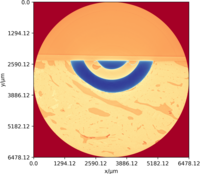
\includegraphics[width=0.96\columnwidth]{770c_pag-full-xy-1x.png}
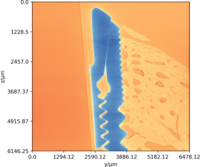
\includegraphics[width=0.96\columnwidth]{770c_pag-full-yz-1x.png}
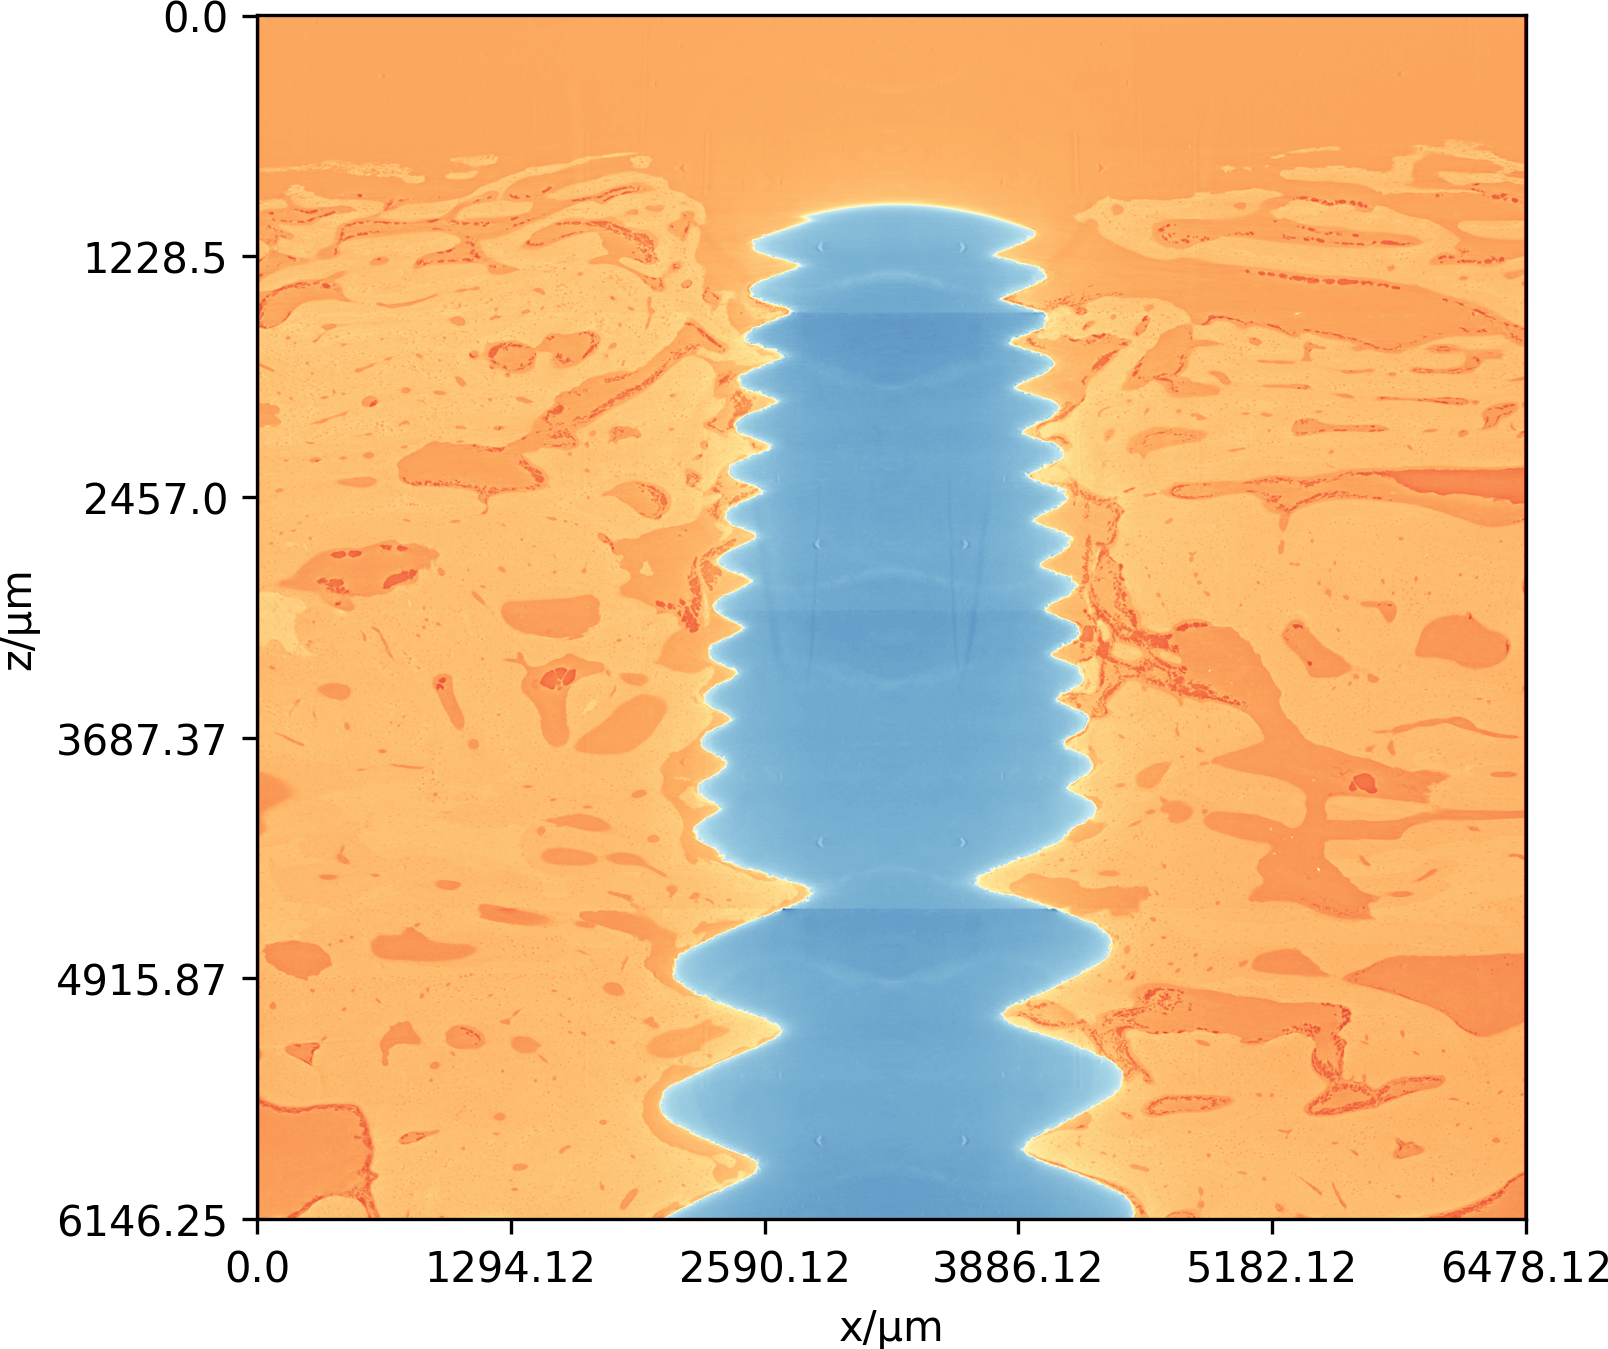
\includegraphics[width=0.96\columnwidth]{770c_pag-full-xz-1x.png}
\caption{Cut sample seen as cross sections in XY, YZ and XZ-planes respectively. A voxel has a size
of 1.875$\mu$m. Red voxels are numerically low, while blue voxels are high.}
\label{fig:3viewsample}
\end{figure}

A cut sample is shown in three different cross sectional views in \Cref{fig:3viewsample}. Each
material has a unique density and thus absorption. The titanium implant shown in blue has a
higher absorption level than bone. Bone material shown in light orange has higher absorption
than its sorrounding dark orange colored regions containing blood vessels tissue, air and resin.

\subsubsection{Data acquisition}

It can be difficult to study and evaluate the bone structure and blood network without destroying
or manipulating the sample. X-ray computed tomography is a widely used tool for non-intrusive medical
imaging. By exposing a subject to X-rays, we can map the linear attentuation coffecient of the passing
rays. Each ray is attenuated relatively to the density and composition of the material it passes.
By rotating either the scanner or the sample we can get a full 3D image representation of the inner
structure of the sample. Each volumetric pixel (voxel) then represents the X-ray attenuation at its
spatial position. We can therefore reliably use X-rays to internally characterise samples in a
non-intrusive and non-destructive manner. Medical CT-scans can provide spatial resolutions on the
order of submillimetre scale \citep{medicalct}. The more modern micro computed tomography ($\mu$CT)
can provide much higher spatial resolution on the micrometre scale \citep{srexptime}.

This work focuses on a data set acquired by Synchrotron Radiation micro-CT (SR$\mu$CT). For this
imaging technique, electrons are accelerated to ultra-relativistic speeds in trajectories directed
by strong magnetic fields. The resulting X-ray beam provides a high photon flux allowing for very
short exposure times \citep{srexptime}. This can help counter Poisson noise from suboptimal photon
count \citep{srnoise}. Contrary to both CT and $\mu$CT, this approach requires a large particle
accelerator, and is not standard medical or laboratory equipment. However, SR$\mu$CT  offers an
even better spatial resolution of up to 0.1 $\mu$m, and much higher image quality due to fewer
distortive X-ray effects. The resulting beams are high in brilliance and collimation, which gives
a very clear signal. Artifacts from beam-hardening are minimized due to synchrotron radiation
X-rays being characeterised by their practially mono-energetic spectrum.

The tomograms prestened here have been acquired at the ID19 beam line at the European Synchrotron
Radiation Facility (ESRF) in Grenoble, France. They were reconstructed\citep{sporring} at the
ID19 beamline. A standard filtered back-projection algorithm was applied via the ESRF in-house developed
software PyHST\citep{pyhst}. PyHST was applied to improve reconstruction quality, hence reducing ring
artefacts, and to reduce the required data volume if necessary~\cite{MIRONE201441}. The
size of the reconstructed tomogram was $2048 \times 2048 \times 1024$ voxels. The segmentation was
performed using VG Studio Max 2.1 (Volume Graphics GHBM, Heidelberg, Germany) also at the ESRF in
Grenoble, France. The tomograms were acquired at 50 KeV.

\subsubsection{Image data}

The full physical size of a sample is about 6.5mm in each direction. Each image sample contains
voxels with a spatial resolution of 1.875$\mu$m. The samples are scanned in chunks of 4-6
sub-volumes through the height of the implant, depending on the initial size of a sample.
For computational purposes, the pixel size has been cropped to be divisible by a power $2^N$ or
more specifically $2^5=32$ was used in our case. This gives a size of $(3456,3456,846)$ pixels
per sub-volume, where the last axis gets stacked for a full volume. This makes the raw dimensions
of a single image containing 4 subvolumes $(3480,3480,3384)$ pixels in total. Before being stacked,
we need to volume match any overlapping regions. The overlaps are only shifted in the last dimension.
This made it possible to find the best overlap by simply minimizing the pixel-wise Eucledian distance
between the volumes. The size of the shifted volumes goes from $846 \rightarrow 810$.

In image \Cref{fig:3viewsample} (YZ and XZ planes) we can clearly see darker edges around the border
of the volume matched subvolumes at their overlaps. This creates an offset which is strongly seen
within the implant, but the large contrast due to very high density, makes this easier to ignore.
Even worse is the contribution of misrepresented voxels in the transitional regions where bone and
tissue contains these jagged edges.

\subsection{Physical effects, noise and artifacts}
\label{sec:physics}

Noise in tomography is unavoidable, and it makes segmentation harder because it further obscures
the boundaries between materials. Matarials may be well separated from certain angles in the
3d-reconstructed image, but overlap from others. Some noise like that corrected by flat-field
correction is very uniformly distributed across images. Some noise is however very spatially
dependent on its sorrounding regions. Knowing the composition and positioning of the materials
being imaged, we can counter some of these effects during segmentation. The noise effects manifest
themselves as numerical shifts in voxel-values as a function of their position. This is a direct
result of a misrepresented attenuation along the axis the X-rays are passing.

This orientation dependency illustrates how voxel intensity values are not globally fixed. How a
certain material is represented in intensity, is highly dependent on its position relative to
neighbouring regions. Especially since this also determines the amount and type of derived noise.
The same material with the same density, can thus be represented at multiple varying intensities
within the same sample.

\begin{figure*}
\centering
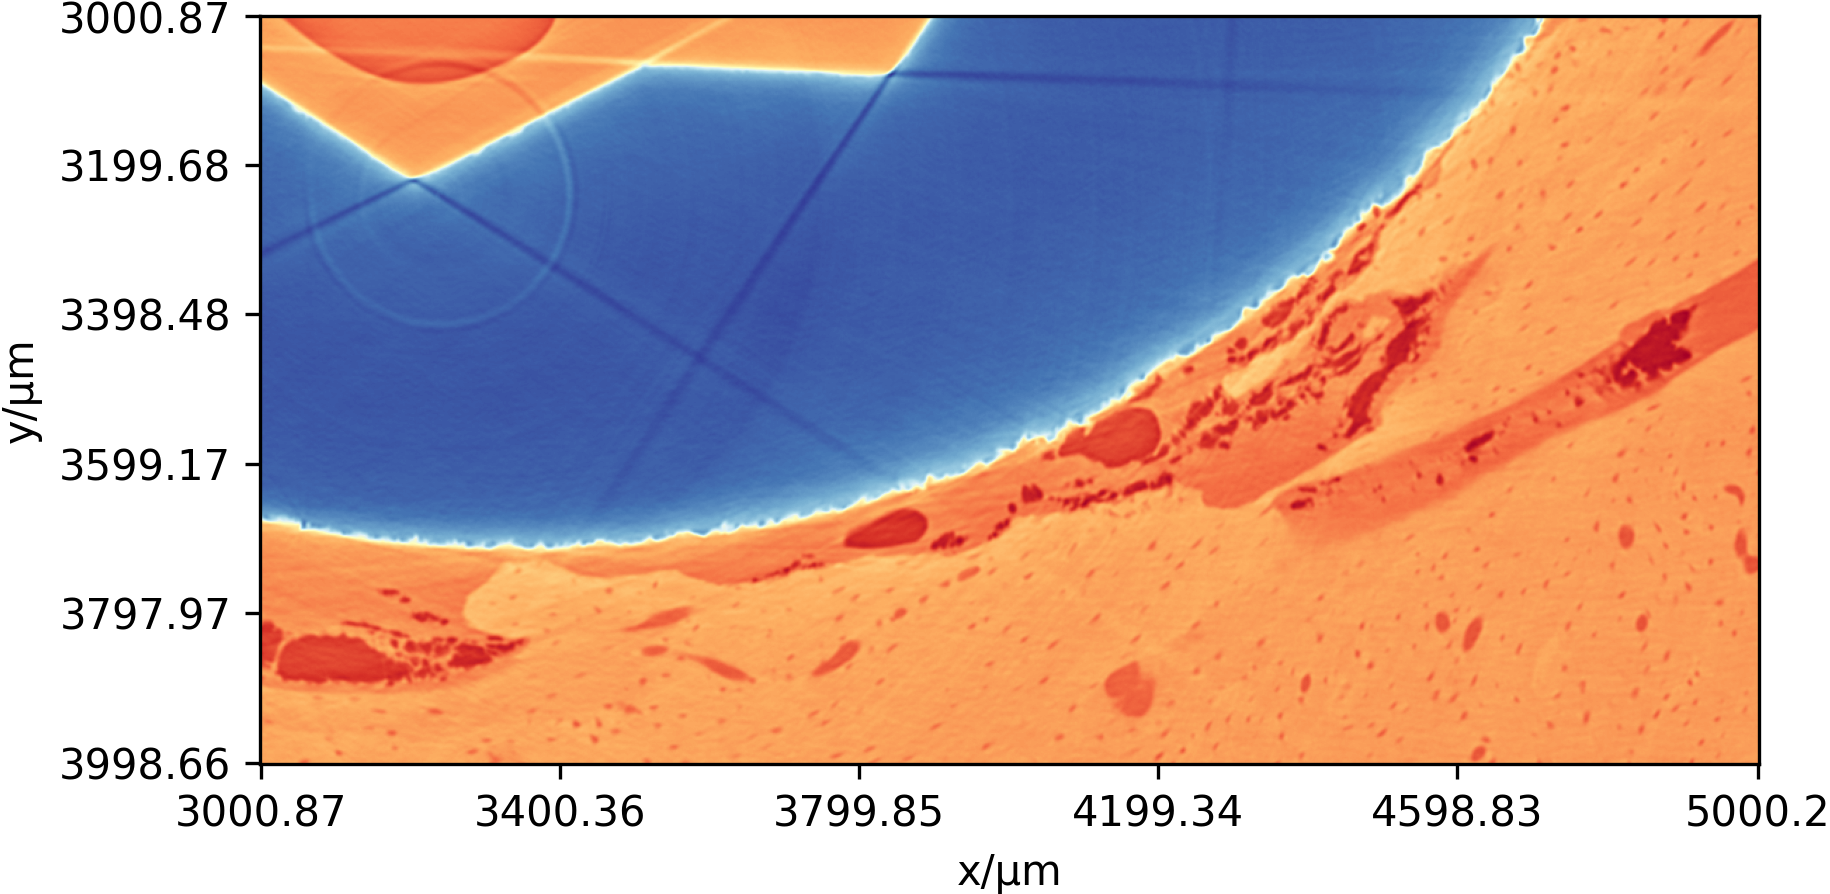
\includegraphics[width=\textwidth]{770c_pag-bic-xy-1x.png}
\caption{Here we see a 1mm x 2mm region of an unscaled image slice in the XY dimension. It highlights
some of the imperfections and noise present in the data. We especially see artifacts within and
around the titanium implant.}
\label{fig:xy-slice}
\end{figure*}

In \Cref{fig:xy-slice} and \Cref{fig:yz-slice} we see zoomed in regions of the XY and YZ planes
of the same sample as shown in \Cref{fig:3viewsample}.
Both planes display a broad selection of the various type of noise sources found in the data.

\begin{figure}
\centering
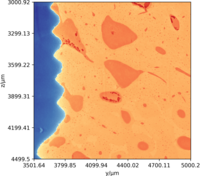
\includegraphics[width=\columnwidth]{770c_pag-bic-yz-1x.png}
\caption{Here we see a 1.5mm x 1.5mm region of an unscaled image slice in the YZ dimension. This
hightlights noise and voxexl effects around the newly formed bone in the micro threaded part of
the titanium implant.}
\label{fig:yz-slice}
\end{figure}


\subsubsection{Ring artifacts}

Looking at the XY-slice in \Cref{fig:xy-slice} we see clear concentric ring artifacts emanating from
the center of the sample, and at strong edges of the titanium implant. It propagates strongly through
the large region of air behind the implant. Compared to the other artifacts mentioned, this effect is
arising from imperfections in the scanner setup. These types of artifacts can typically come from
uncalibrated or defect adjacent detector elements. For synchrotron radiation sources it can also
occur from shifts and vibrations in the monochromator crystal \citep{ringartifacts}.

\subsubsection{Projection artifacts}

Bright streaks with strong edges are seen from the sharp corners of the titanium implant. When
doing back projection, the symmetry breaking is seen as smeared lines across the sample. This
can occur from the high pass filter used during filtered back projection, which exaggerates the
differences between adjacent elements \citep{ctnoise}.

\subsubsection{Compton scattering}

Lower energy rays contribute mostly with noise from scattering effects. A ray will propagate through
a material, get scattered and diffract from its initial trajectory. This gives a misrepresentation
of the attenuation along its initial trajectory. The artefacts seen from scattering are similar in
nature to those formed by beam hardening. This is because both effectively reduce the measured
attenuation. For energy levels of above 50KeV relevant for the data presented here, Compton
scattering is the dominating type \citep{compton}. The scattering occurs due to photon-electron
interaction between X-ray beam and the material it passes through. Like beam-hardening, scattering
will cause dark streaks across the image, where attenuation was highest.

\subsection{Beam hardening}\label{sec:beam-hardening}

Medical CT and $\mu$CT both utilize poly-energetic beams, which can cause artifacts around high
density regions. This effect is called beam-hardening \citep{beamhardening}, and occurs when rays
with lower energy are attenuated more frequently, thus shifting the remaining photon energy to a
higher effective average value. This offsets the local contrast, by overestimating the attenuation,
leaving lighter spots on the image. Many types of artifacts will typically be present in these
setups, but most are taken into account by calibration using phantoms and pre-hardening the beam
before it reaches the sample. Pre-hardening of the beam is done using filters that attenuate the
softest rays. Due to its common usage, various metal artifact reduction (MAR) software exists to
account for noise and imperfections during reconstruction \citep{mar1}\citep{mar2}.

Despite the practially mono-energetic rays from SR$\mu$CT, the source initially generates a
polychromatic spectrum. During monochromatisation the resulting spectrum can still contain
corrupted harmonic components. Only a few percent corruption is enough to produce strong
artifacts, although monochromatisation is typically done in multiple layers \citep{srnoise}.
It can not trivially be rejected that some noise does occur from poly-energetic incident radiation.
Two distinct effects typically seen as a result of beam-hardening are in dark and bright streaks
and cupping artifacts in high density regions.

\subsubsection{Dark and bright streaks}

Streaking artifacts occur at the dense implant region, but also in the transition from bone to softer
tissue. This effect is mostly seen in regions of large heterogeneity. When X-ray beams pass at angles
containing multiple dense obstacles, the beam is hardened more. Then for angles with fewer dense
obstacles the energy spectrum is preserved better. This produced the dark and bright streaks seen in
\Cref{fig:xy-slice}.

For a hardened beam, softer x-rays are absorbed instead of successfully penetrating the object,
and will not contribute to image formation. High density structures such as the titanium implant
break the isotropy, making the projected X-ray mean energy spectrum dependent on incident orientation
\citep{srnoise}.

\subsubsection{Cupping effect}

A common artefact that occurs when beams pass more homogeneous cylindrical objects. Since beams
passing the middle will traverse more material compared to the edges, the beam is hardened more
towards the center and intensity becomes lower as a result. This can manifest itself in what
errnoeously looks to be dense peripheral regions at the edges.

\subsection{Phase contrast}

Phase contrast is an effect whose consequences are not very unlike those of beam-hardening.
Although used as an advantage in holotomography\citep{holotomography} and phase contrast tomography\citep{phasecontrast},
it induces noise in regular tomography such as used here. It typically results in fringes around edges
of regions within the image\citep{srnoise}. Similar to dark and bright streaks mentioned above,
they show as misrepresentations of the voxel values. In our case we see them especially at the
transitional edges between the titanium implant and the biological tissue and bone.

%Partial volume artifacts which are dependent on the voxel size and are mentioned briefly by Neldam et al.

%%% Local Variables:
%%% mode: latex
%%% TeX-master: "main"
%%% End:
